 %	Main Document

\documentclass[
	12pt,
	BCOR=5mm,
	DIV=12,
	headinclude=on,
	footinclude=off,
	parskip=half,
	bibliography=totoc,
	listof=entryprefix,
	toc=listof,
	pointlessnumbers,
	plainfootsepline]{scrreprt}

% include configuration file
% !TEX root =  master.tex

% language, font, colors
\usepackage[ngerman]{babel}
\usepackage[utf8]{inputenc}
\usepackage[german=quotes]{csquotes} 	% correct quotes using \enquote{}
\usepackage[T1]{fontenc}
\usepackage{lmodern} % latin modern font
\usepackage[onehalfspacing]{setspace}
\usepackage{xcolor}

% hyperlinks
%\PassOptionsToPackage{hyphens}{url}
\usepackage[hidelinks=true]{hyperref}

% commands for author and title
\newcommand{\TitelDerArbeit}[1]{\def\DerTitelDerArbeit{#1}\hypersetup{pdftitle={#1}}}
\newcommand{\AutorDerArbeit}[1]{\def\DerAutorDerArbeit{#1}\hypersetup{pdfauthor={#1}}}
\newcommand{\Firma}[1]{\def\DerNameDerFirma{#1}}
\newcommand{\Kurs}[1]{\def\DieKursbezeichnung{#1}}


%\usepackage{microtype}% verbesserter Randausgleich
%\setlength\emergencystretch{1em}
% correct superscripts
\usepackage{fnpct}

\usepackage{footnote}
\usepackage{rotating}

% calc
\usepackage{calc} % Used for extra space below footsepline

% bibliography settings
% author-year-style with footnotes (Chicago)
\usepackage[backend=biber, autocite=footnote, style=authoryear, dashed=false]{biblatex}
\AdaptNoteOpt\footcite\multfootcite
\AdaptNoteOpt\autocite\multautocite

\DefineBibliographyStrings{ngerman}{  % change \ua to et al. (german only!)
	andothers = {{et\,al\adddot}},
}


% Command to output section title headings
\newcommand{\cvsect}[1]{% The only parameter is the section text
	\vspace{\baselineskip} % Whitespace before the section title
	\colorbox{black}{\textcolor{white}{\MakeUppercase{\textbf{#1}}}}\\% Section title
}

\newcounter{barcount}

% Environment to hold a new bar chart
\newenvironment{barchart}[1]{ % The only parameter is the maximum bar width, in cm
	\newcommand{\barwidth}{0.35}
	\newcommand{\barsep}{0.55}
	
	% Command to add a bar to the bar chart
	\newcommand{\baritem}[2]{ % The first argument is the bar label and the second is the percentage the current bar should take up of the total width
		\pgfmathparse{##2}
		\let\perc\pgfmathresult
		
		\pgfmathparse{#1}
		\let\barsize\pgfmathresult
		
		\pgfmathparse{\barsize*##2/5}
		\let\barone\pgfmathresult
		
		\pgfmathparse{(\barwidth*\thebarcount)+(\barsep*\thebarcount)}
		\let\barx\pgfmathresult
		
		\filldraw[fill=none, draw=black!] (0,-\barx) rectangle (5,-\barx-\barwidth);
		\filldraw[fill=black!90, draw=black!90] (0,-\barx) rectangle (\barone,-\barx-\barwidth);
		
		\node [label=180:{\textcolor{black}{##1: ##2/5}}] at (0,-\barx-0.175) {};
		\addtocounter{barcount}{1}
	}

	\newcommand{\baritemNL}[2]{ % The first argument is the bar label and the second is the percentage the current bar should take up of the total width
		\pgfmathparse{##2}
		\let\perc\pgfmathresult
		
		\pgfmathparse{#1}
		\let\barsize\pgfmathresult
		
		\pgfmathparse{\barsize*##2/5}
		\let\barone\pgfmathresult
		
		\pgfmathparse{(\barwidth*\thebarcount)+(\barsep*\thebarcount)}
		\let\barx\pgfmathresult
		
		\filldraw[fill=none, draw=black!] (0,-\barx) rectangle (5,-\barx-\barwidth);
		\filldraw[fill=black!90, draw=black!90] (0,-\barx) rectangle (\barone,-\barx-\barwidth);
		
		\node [label=180:{}] at (0,-\barx) {};
		\addtocounter{barcount}{1}
	}

	\begin{tikzpicture}
	\setcounter{barcount}{0}
}{
	\end{tikzpicture}
	\vspace{0.3cm}
}

\usepackage{tikz} % Required for creating the plots
\usetikzlibrary{shapes, backgrounds}
\tikzset{x=1cm, y=1cm} % Default tikz units

%%% Uncomment the following lines to support hard URL breaks in bibliography 
\apptocmd{\UrlBreaks}{\do\f\do\m}{}{}
\setcounter{biburllcpenalty}{9000}% Kleinbuchstaben
\setcounter{biburlucpenalty}{9000}% Großbuchstaben

\setlength{\bibparsep}{\parskip}	% add some space between biblatex entries in the bibliography
\addbibresource{bibliography-martin.bib}	% add file bibliography.bib as biblatex resource
\addbibresource{bibliography-rene.bib}	% add file bibliography.bib as biblatex resource
\addbibresource{bibliography-sascha.bib}	% add file bibliography.bib as biblatex resource
\addbibresource{bibliography-niko.bib}	% add file bibliography.bib as biblatex resource
\addbibresource{bibliography-julian.bib}	% add file bibliography.bib as biblatex resource
\addbibresource{bibliography-erik.bib}	% add file bibliography.bib as biblatex resource
% footnotes (count footnotes over chapters)
\usepackage{chngcntr}
\counterwithout{footnote}{chapter}

% acronyms
\makeatletter
\usepackage[printonlyused]{acronym}
\@ifpackagelater{acronym}{2015/03/20}
  {%
    \renewcommand*{\aclabelfont}[1]{\textbf{\textsf{\acsfont{#1}}}}
  }%
  {%
  }%
\makeatother

% listings
\usepackage{listings}
\renewcommand{\lstlistingname}{Quelltext}
\renewcommand{\lstlistlistingname}{Quelltextverzeichnis}

%% More configuration for listings is in configlistings.tex %%


% extra packages
\usepackage{graphicx}			% use various graphics formats
\usepackage[german]{varioref}	% nicer references \vref
\usepackage{caption}			% better captions
\usepackage{booktabs}			% nicer tabs
\usepackage{array}
\usepackage{pdfpages}			% for signed ewerkl
%\usepackage{import}				% better import of section in several files
\usepackage{subfigure}

% table stuff
\newcolumntype{L}[1]{>{\raggedright\let\newline\\\arraybackslash\hspace{0pt}}m{#1}} % combines l and p
\newcolumntype{C}[1]{>{\centering\let\newline\\\arraybackslash\hspace{0pt}}m{#1}} % combines c and p
\newcolumntype{R}[1]{>{\raggedleft\let\newline\\\arraybackslash\hspace{0pt}}m{#1}} % combines r and p

% funktioniert aktuell nicht wie normal -> muss man nochmal drüber schauen.. oder ersetzen
\usepackage{tabularx}

% page header/footer
\RequirePackage{scrlfile}
\ReplacePackage{scrpage2}{scrlayer-scrpage}
\RequirePackage[automark,headsepline,footsepline]{scrpage2}
\pagestyle{scrheadings}
\renewcommand*{\pnumfont}{\upshape\sffamily}
\renewcommand*{\headfont}{\upshape\sffamily}
\renewcommand*{\footfont}{\upshape\sffamily}
\renewcommand{\chaptermarkformat}{}
\RedeclareSectionCommand[beforeskip=0pt]{chapter}
\clearscrheadfoot

\ifoot[\rule{0pt}{\ht\strutbox+\dp\strutbox}DHBW Mannheim]{\rule{0pt}{\ht\strutbox+\dp\strutbox}DHBW Mannheim}
\ofoot[\rule{0pt}{\ht\strutbox+\dp\strutbox}\pagemark]{\rule{0pt}{\ht\strutbox+\dp\strutbox}\pagemark}

\ohead{\headmark}

% highlight notes as not yet finished
\newenvironment{note}{\color{gray}}{}

\usepackage{todonotes}
\usepackage{xspace}% http://ctan.org/pkg/xspace
\usepackage{fontawesome5}
\usepackage{float} % !important for figure position

\usepackage{pifont} % for description
% !TEX root =  master.tex

% colors
\definecolor{javared}{rgb}{0.6,0,0} % for strings
\definecolor{javagreen}{rgb}{0.25,0.5,0.35} % comments
\definecolor{javapurple}{rgb}{0.5,0,0.35} % keywords
\definecolor{javadocblue}{rgb}{0.25,0.35,0.75} % javadoc

\colorlet{jsonPunct}{red!60!black}
\definecolor{jsonBackground}{HTML}{EEEEEE}
\definecolor{jsonDelim}{RGB}{20,105,176}
\colorlet{jsonNumb}{magenta!60!black}

\definecolor{xmlGray}{rgb}{0.4,0.4,0.4}
\definecolor{xmlDarkblue}{rgb}{0.0,0.0,0.6}
\definecolor{xmlCyan}{rgb}{0.0,0.6,0.6}

\definecolor{jsBackground}{RGB}{250,250,255}
\definecolor{jsString}    {RGB}{ 16,160, 60}

\definecolor{cssKeyword}{RGB}{ 10,100,160}
\definecolor{cssClass}  {RGB}{200,120, 10}

% general style
\lstset{
	basicstyle=\ttfamily\footnotesize,
	backgroundcolor=\color{jsBackground},
	numbers=left,
	numberstyle=\scriptsize\color{black},
	stepnumber=1,
	numbersep=10pt,
	showspaces=false,
	showstringspaces=false,
	breaklines=true,
	tabsize=2,
	captionpos=b,
	literate=
	{Ö}{{\"O}}1
	{Ä}{{\"A}}1
	{Ü}{{\"U}}1
	{ß}{{\ss}}1
	{ü}{{\"u}}1
	{ä}{{\"a}}1
	{ö}{{\"o}}1
}

% Java
\lstdefinestyle{lstJava}
{
	language=Java,
	keywordstyle=\color{javapurple}\bfseries,
	stringstyle=\color{javared},
	commentstyle=\color{javagreen},
	morecomment=[s][\color{javadocblue}]{/**}{*/},
	tabsize=1
}

% JSON
\lstdefinelanguage{json}{
	literate=
	*{0}{{{\color{jsonNumb}0}}}{1}
	{1}{{{\color{jsonNumb}1}}}{1}
	{2}{{{\color{jsonNumb}2}}}{1}
	{3}{{{\color{jsonNumb}3}}}{1}
	{4}{{{\color{jsonNumb}4}}}{1}
	{5}{{{\color{jsonNumb}5}}}{1}
	{6}{{{\color{jsonNumb}6}}}{1}
	{7}{{{\color{jsonNumb}7}}}{1}
	{8}{{{\color{jsonNumb}8}}}{1}
	{9}{{{\color{jsonNumb}9}}}{1}
	{:}{{{\color{jsonPunct}{:}}}}{1}
	{,}{{{\color{jsonPunct}{,}}}}{1}
	{\{}{{{\color{jsonDelim}{\{}}}}{1}
	{\}}{{{\color{jsonDelim}{\}}}}}{1}
	{[}{{{\color{jsonDelim}{[}}}}{1}
	{]}{{{\color{jsonDelim}{]}}}}{1}
}

% XML
\lstdefinelanguage{XML}
{
	morestring=[b]",
	morestring=[s]{>}{<},
	morecomment=[s]{<?}{?>},
	stringstyle=\color{xmlGray},
	identifierstyle=\color{xmlDarkblue},
	keywordstyle=\color{xmlCyan},
	morekeywords={xmlns,version,type}
}

% JavaScript
\lstdefinelanguage{JavaScript}
{
	backgroundcolor=\color{jsBackground},
	keywordstyle=\color{blue}\bfseries,
	stringstyle=\color{jsString},
	commentstyle=\color{gray},
	morestring=[b]",
	morecomment=[l][\color{gray}]{//},
	morecomment=[s][\color{gray}]{/*}{*/},
	morekeywords={break,case,const,continue,else,false,for,function,if,in,new,null,switch,this,true,var,while}
}

% HTML
\lstdefinestyle{lstHTML}
{
	language=HTML,
	keywordstyle=\color{blue}\bfseries,
	commentstyle=\color{gray}\itshape,
	morecomment=[s][\color{gray}]{<!--}{-->},
%	stringstyle=\color{jsString}
	escapeinside=``
}

% CSS
\lstdefinestyle{lstCSS}
{
	keywordstyle=\color{cssKeyword}\bfseries,
	commentstyle=\color{gray}\itshape,
	morecomment=[s][\color{gray}]{/*}{*/},
%	morecomment=[s][\color{cssClass}]{.}{ \{},
	alsoletter=-,
	morekeywords={border,background-color}
}

%lstinline
\def\jinline{\lstinline[basicstyle=\ttfamily,keywordstyle={}, language=JAVA]}
\def\sinline{\lstinline[basicstyle=\ttfamily,keywordstyle={}, language=SQL]}

% create free field for chapter
\makeatletter
\newcommand{\freechapterauthor}[1]{%
	{\parindent0pt\vspace*{-25pt}%
		\linespread{1.1}\large\scshape#1%
		\par\nobreak\vspace*{35pt}}
	\@afterheading%
}
\makeatother

% create author for chapter
\makeatletter
\newcommand{\chapterauthor}[1]{%
	{\parindent0pt\vspace*{-25pt}%
		\linespread{1.1}\large\scshape Autor: #1%
		\par\nobreak\vspace*{35pt}}
	\@afterheading%
}
\makeatother

% create multiple author for chapter
\makeatletter
\newcommand{\chaptermulitpleauthor}[2]{%
	{\parindent0pt\vspace*{-25pt}%
		\linespread{1.1}\large\scshape Autoren: #1, #2%
		\par\nobreak\vspace*{35pt}}
	\@afterheading%
}
\makeatother

% create free for section
\makeatletter
\newcommand{\freeauthorsection}[1]{%
	{\parindent0pt\vspace*{0 pt}%
		\linespread{1.1}\scshape#1%
		\par\nobreak\vspace*{15pt}}
	\@afterheading%
}
\makeatother

% create author for section
\makeatletter
\newcommand{\authorsection}[1]{%
	{\parindent0pt\vspace*{0 pt}%
		\linespread{1.1}\scshape Autor: #1%
		\par\nobreak\vspace*{15pt}}
	\@afterheading%
}
\makeatother

% create multiple author for section
\makeatletter
\newcommand{\multipleauthorsection}[2]{%
	{\parindent0pt\vspace*{0 pt}%
		\linespread{1.1}\scshape Autoren: #1, #2%
		\par\nobreak\vspace*{15pt}}
	\@afterheading%
}
\makeatother

% !TEX root =  master.tex

\newcommand{\authorSG}{Sascha Görnert}
\newcommand{\authorNL}{Niko Lockenvitz}
\newcommand{\authorRF}{Rene Fischer}
\newcommand{\authorEJ}{Erik Jansky}
\newcommand{\authorMS}{Martin Sandig}

\newcommand{\authorGP}{Gerrit Pollkläsener}
\newcommand{\quelle}{\footnotesize Quelle: }

\newcommand{\quelleScreenshot}{\footnotesize Quelle: Bildschirmaufnahme}

\newcommand{\zb}{z.~B.\xspace}

\newcommand{\ua}{u.~a.\xspace}

\newcommand{\Zb}{Z.~B.\xspace}

\newcommand{\martin}{bzw.\xspace}

\newcommand{\engl}[1]{(\emph{engl. #1})}

\newcommand{\props}{\jinline|props|\xspace}

\newcommand{\state}{\jinline|state|\xspace}

\newcommand{\render}{\jinline|render|\xspace}

\newcommand{\cwm}{\jinline|componentWillMount|\xspace}

\newcommand{\cdm}{\jinline|componentDidMount|\xspace}

\newcommand{\exampleState}{\jinline|this.setState(\{ name: value \})|\xspace}

\newcommand{\myRefGeneral}[1]{\vref{#1}, \enquote{\nameref{#1}}}

\newcommand{\figma}{\footnotesize Quelle: Eigene Darstellung mittels \url{https://www.figma.com/}}

% numbers

\newcommand{\HugoBlue}{\Large\color{blue}}

\newcommand{\desOne}{{\HugoBlue\ding{182}}\xspace}

\newcommand{\desTwo}{{\HugoBlue\ding{183}}\xspace}

\newcommand{\desThree}{{\HugoBlue\ding{184}}\xspace}

\newcommand{\desFour}{{\HugoBlue\ding{185}}\xspace}

\newcommand{\desFive}{{\HugoBlue\ding{186}}\xspace}

\newcommand{\desSix}{{\HugoBlue\ding{187}}\xspace}

\newcommand{\desSeven}{{\HugoBlue\ding{188}}\xspace}

\newcommand{\desEight}{{\HugoBlue\ding{189}}\xspace}

\newcommand{\desNine}{{\HugoBlue\ding{190}}\xspace}

\begin{document}

% set some information (title, author, ...)
\TitelDerArbeit{Konzeption und Implementierung einer Webanwendung zum Erstellen, Durchführen und Auswerten von Umfragen} % Hochschulumfeld?
\AutorDerArbeit{\authorSG, \authorRF, \authorMS, \authorEJ, \authorNL, \authorJR}
\Firma{DER Touristik Deutschland GmbH, Technische Universität Kaiserslautern, SAP SE}
\Kurs{WWI 17 SE B}

\begin{titlepage}

\begin{minipage}{\textwidth}
	\vspace{-2cm}
	\noindent
	\includegraphics[height=0.1\linewidth]{img/logos/der}
	\hfill
	\includegraphics[height=0.1\linewidth]{img/logos/tukl}
	\hfill
	\includegraphics[height=0.1\linewidth]{img/logos/sap}
	\hfill
	\includegraphics[height=0.1\linewidth]{img/logos/dhbw}
\end{minipage}

\vspace{1em}
\sffamily

\begin{center}
	\textsf{\large{}Duale Hochschule Baden-Württemberg\\[1.5mm] Mannheim}\\[2em]
	\textsf{\textbf{\Large{}Seminararbeit}}\\[3mm]
	\textsf{\textbf{\DerTitelDerArbeit}}\\[1.5cm]
	\textsf{\textbf{\Large{}Studiengang Wirtschaftsinformatik}\\[3mm] \textsf{Studienrichtung Software Engineering}}
	
	\vspace{3em}
	\vfill

	\begin{minipage}{\textwidth}
	
		\begin{tabbing}
			Bearbeitungszeitraum: \hspace{0.85cm}\=\kill
			Verfasser: \> \authorSG, 2716910 \\
			\> DER Touristik GmbH \\
			\> \\
			\> \authorRF, 8703049 \\
			\> Technische Universität Kaiserslautern \\
			\> \\
			\> \authorGP, 1930724 \\
			\> SAP SE \\
			\> \\
			\> \authorEJ, 5980253 \\
			\> SAP SE \\
			\> \\
			\> \authorNL, 1308674 \\
			\> SAP SE \\
			\> \\[1.5mm]
			Kurs: \> \DieKursbezeichnung \\[1.5mm]
			Bearbeitungszeitraum: \> 19.11.2018 -- 15.02.2019
	\end{tabbing}

	\end{minipage}

\end{center}

\end{titlepage}

\pagenumbering{roman}
\normalfont

% table of contents
\clearpage
\pdfbookmark{Inhaltsverzeichnis}{toc-bookmark}
\tableofcontents

% figures
\listoffigures

% tables
%\listoftables

% listings (source code)
\lstlistoflistings

% acronyms
\clearpage
\chapter*{Abkürzungsverzeichnis}
\addcontentsline{toc}{chapter}{Abkürzungsverzeichnis}

\begin{acronym}[A23456789012] % longest acronym for correct indentation
	\acro{A23456789012}{This is just for indentation}

	\acro{AJAX}{Asynchronous JavaScript and \acs{XML}}
	\acro{API}{Application Programming Interface}
	\acro{CRUD}{Create, Read, Update, Delete}
	\acro{CSS}{Cascading Style Sheets}
	\acro{DAO}{Data Access Object}
	\acro{DBMS}{Datenbankmanagementsystem}
	\acro{DOM}{Document Object Model}
	\acro{DTO}{Data Transfer Object}
	\acro{ER-Modell}{Entity-Relationship-Modell}
	\acro{FSK}{Freiwillige Selbstkontrolle der Filmwirtschaft}
	\acro{HTML}{Hypertext Markup Language}
	\acro{HTTP}{Hypertext Transfer Protocol}
	\acro{HTTPS}{Hypertext Transfer Protocol Secure}
	\acro{IDE}{Integrated Development Environment}
	\acro{JPA}{Java Persistence \acs{API}}
	\acro{JPQL}{Java Persistence Query Language}
	\acro{JSON}{JavaScript Object Notation}
	\acro{ORM}{Objektrelationaler Mapper}
	\acrodefplural{ORM}{Objektrelationale Mapper}
	\acro{POJO}{Plain Old Java Object}
	\acro{QR-Code}{Quick Response Code}
	\acro{RDBMS}{Re\-la\-tio\-nal Database Management System}
	\acro{REST}{Representational State Transfer}
	\acro{SQL}{Structured Query Language}
	\acro{URI}{Uniform Resource Identifier}
	\acro{URL}{Uniform Resource Locator}
	\acro{XML}{Extensible Markup Language}
\end{acronym}

\ohead{Abkürzungsverzeichnis}

%--------------------------------
% Content
%--------------------------------
\clearpage
\ihead{\chaptername~\thechapter}
\ohead{\headmark}
\pagenumbering{arabic}

\chapter{Einleitung}
\label{ch:einleitung}
% !TEX root =  ../../master.tex
\section{Motivation und Zielsetzung}

In der heutigen digitalisierten Welt sind Online-Umfragen ein bewährtes Mittel der Sozialforschung.
Das beste Beispiel hierfür ist das Unternehmen Alphabet Inc., welches durch seine Google-Umfrage-Applikation Android-Nutzern regelmäßig Umfragen unterbreitet. 
Hiermit verbessert es nicht nur die eigenen Produkte wie YouTube, sondern versucht auch Werbevorschläge zu optimieren.
Auch für die \acs{DHBW} Mannheim ist eine solche Möglichkeit zur Sozialforschung von großem Nutzen.
Aus diesem Grund soll im Rahmen dieser Seminararbeit eine eigene Anwendung für Online-Umfragen entwickelt werden, sodass die \acs{DHBW} in Zukunft ohne die Nutzung von Drittanbieter-Software auskommen kann.
Damit soll gewährleistet werden, dass alle erhobenen Daten lediglich zur Sozialforschung der \acs{DHBW} Mannheim verwendet werden.

So liegt das Ziel der Arbeit auf der Gestaltung und Umsetzung einer Webanwendung, die es ermöglicht, Umfragen zu erstellen, zu verwalten und auszuwerten.
Dabei sollen Dozenten mithilfe der Anwendung die Möglichkeit haben, Umfragen für ihre Studierenden zu erstellen.
Diese haben dadurch die Chance, ihre Meinung zur Vorlesung mitzuteilen, Gelerntes zu verinnerlichen oder auch um Anmerkungen zu gestellten Fragen zu geben.
Die zu entwickelnde Plattform soll dabei auch die Möglichkeit bieten, solche Umfragen in verschiedenen Kursen zu wiederholen und die Ergebnisse der Umfragen betrachten zu können.
Auf spezifische Fragen und Probleme soll somit gezielter eingegangen werden können.
Außerdem soll damit der Lernfortschritt der Studierenden überblickt werden.
Grundlegend dient die Umfrage-Anwendung ebenfalls als Datengrundlage für den großen Bereich der Learning Analytics und soll die Datenerhebung dazu erleichtern.


Diese Dokumentation beschreibt die im Umfang des Moduls Integrationsseminar entwickelte Umfrageapplikation \enquote{MyLA} der Gruppe um Sascha Görnert (DER), Rene-Pascal Fischer (TUK), Erik Jansky (SAP), Niko Lockenvitz (SAP) sowie Martin Sandig (SAP).
% TODO
Der Name Julian Rolle (SAP) steht auch auf dieser Arbeit.

% !TEX root =  ../../master.tex
\section{Aufbau}

\textit{\textbf{Bemerkung der Autoren:}
Diese Arbeit bzw. dieses Dokument erhebt nicht den Anspruch einer wissenschaftlichen Arbeit, sondern spiegelt lediglich den Entwicklungsprozess der erstellten Software wieder. 
Hierzu werden entsprechende Grundlagen vermittelt.}

Zunächst werden die theoretischen Grundlagen, wie \ac{REST} in den Kapitel \vref{sec:theoretisch}, den Grundlagenteil, gelegt.
Anschließend daran folgen Ausführungen zu den Techniken hinter Microservices und Prototyping.
Weiterhin werden die theoretischen Erläuterungen mit der Dokumentation von dem Konzept der relationalen Datenbank und Fragebogentheoretischen Ausführungen. 
Abschließend wird auf die Idee und die Verwendung von Learning Analytics im allgemeinen eingegangen. 

Im Folgenden werden in Kapitel \vref{sec:technisch}, die technischen Grundlagen gelegt, um ein Verständnis für die verwendeten Technologien zu schaffen. 
Den Anfang bildet die Technologie Docker, dabei wird auf die Container-Virtualisierung eingegangen und diese für die Verwendung evaluiert. % ??
Um einen Bezug zu den theoretischen Grundlagen zu haben, bildet das Kapitel über PostgreSQL ein reales Anwendungsbeispiel für eine relationale Datenbank.  
Schlussendlich werden die Grundlagen mit einem Ausblick in das verwendete Front-End-Framework, React, abgeschlossen. 

Darauf folgend wird im Kaptitel \vref{ch:analyse} eine Ist-Analyse der bestehenden Learning-Analytics-Software durchgeführt. 
Dabei wird näher darauf eingegangen, inwiefern die vorherige Lösung in die neue Implementierung eines Umfragetools für Studierende und Dozierende mit einwirken kann. 
Um einen klar abgegrenzten Start in die Implementierung zu legen, werden die Anforderungen an das neue Tool detailliert aufgeführt. 
Nachdem die Anforderungen evaluiert sind, werden alternative bestehende Lösungen analysiert und abgegerenzt, inwiefern die Konzepte aus anderen Lösungen mit in die eigene Implementierung integriert werden können. 
Zum Abschluss der Analyse werden drei Personas als mögliche Nutzer der Software vorgestellt.

In dem Kapitel \vref{ch:konzeption}, wird auf die Konzeption eingegangen. 
Zuerst wird gesamtheitlich auf das Konzept eingegangen, inwiefern die Teile der Software miteinander zusammenspielen sollen. 
Anschließend werden konzeptionell die einzelnen Komponenten Server, Client und Sicherheit, beschreiben. 

Nach der ausführlichen Erläuterung der Konzeption wird nun in Kapitel \vref{ch:implementierung} auf die Implementierung dieser Komponenten eingegangen. 
Ebenfalls wird auf das verwendete Docker-Netzwerk eingegangen, welches die Komponenten miteinander verbindet und die Kommunikation dieser in einem abgesicherten System ermöglicht.
Die Implementierung orientiert sich dabei an die konzeptionierten Ideen, jedoch sind im Verlauf des Projektes einige Abweichungen entstanden.
Diese Abweichungen wurde auf Grund von Zeitgründen nicht noch einmal in den vorgesehen Mock-Ups angepasst.

Nach dem erfolgreichen Durchführen des Projektes wird ein Nutzerhandbuch im Kapitel \vref{ch:nutzerhandbuch} vorgestellt, in dem wesentliche Nutzungsaspekte im Detail erläutert werden.
Dabei wird beispielsweise beschrieben, wie Umfragersteller sich bei der Software registrieren und anmelden können.

Die Dokumentation wird dem Kapitel \vref{ch:ausblick} zum Abschluss gebracht. 
Durch ein Fazit zur Gruppen- und Seminararbeit wird abschließend ein Überblick zur Arbeit gegeben. 
Um den weiteren Verlauf und die möglichen Anhaltspunkte für Weiterentwicklungen abzugrenzen, wird der Abschluss mit einem Ausblick gemacht.

\chapter{Grundlagen}
\label{ch:grundlagen}
% !TEX root =  ../../master.tex
\section{Theoretische Grundlagen}
% !TEX root =  ../theoretisch.tex
\subsection{Representational State Transfer}

Die Technologie der Schnittstellen zur Kommunikation zwischen Softwaresystemen hat sich im Verlauf der Jahre stetig geändert. 
Hierzu gibt es verschiedenste Arten von Schnittstellen. 
Gerade die bekannten Internetunternehmen wie Google\autocite{MS-GoogleLLC.2020}, Twitter\autocite{MS-TwitterInc..01.03.2020} oder Microsoft\autocite{MS-MicrosoftCorporation.21.05.2018} bieten teilweise dutzende öffentliche Schnittstellen in Form von \acp{API} an.

Der wohl bekannteste und derzeit aktuellste Schnittstellentyp von \acp{API} sind auf dem \ac{REST}-Paradigma basierende Schnittstellen. 
Dieses Paradigma bzw. diese Architekturweise wurde von Roy Thomas Fielding in seiner Dissertation\autocite{MS-Fielding.} vorgestellt und wurde ursprünglich für verteilte hypermediale Systeme entworfen. 
\ac{REST} ist selbst kein Standard, sondern beschreibt sechs Prinzipien für eine Web-Architektur. 
Das erste Prinzip beruht auf einer Client-Server-Architektur, bei der die Benutzerschnittstelle von der Datenhaltung entkoppelt wird.
Dadurch soll eine höhere Skalierbarkeit und Portabilität für verschiedene Plattformen gewährleistet werden.
Ebenfalls ist hierdurch eine unabhängige Weiterentwicklung der Komponenten möglich. 
Das zweite Prinzip bezieht sich auf die Zustandslosigkeit (engl. \enquote{stateless}). 
Damit ist gemeint, dass alle Anfragen vom Client an den Server stets alle nötigen Informationen beinhalten, die der Server benötigt. 
Dieser arbeitet somit kontextlos und muss sich keine Sitzungsinformationen speichern. 
Alle Anfragen können somit atomar und isoliert voneinander betrachtet werden. Dadurch erhöht sich die Zuverlässigkeit sowie ebenfalls die Skalierbarkeit.

Der dritte Grundsatz nach \citeauthor{MS-Fielding.} ist der Cache. 
Damit ist das Zwischenspeichern bzw. das Vorhalten von Daten gemeint, die schon einmal benutzt wurden. 
Laut diesem Prinzip sollen die Daten als \enquote{cachable} oder \enquote{not cachable} markiert werden. 
Dadurch soll die gesamte Netzwerkeffizienz verbessert bzw. die Netzwerkauslastung verringert werden. 
Dem Vorteil der Performanceverbesserung steht jedoch die Problematik, das Original auf dem Server mit dem Inhalt des Caches synchron zu halten, gegenüber. 
Veraltete Daten im Cache können gegebenenfalls zu fehlerhaften Ergebnissen führen. 
Das nächste Prinzip bezieht sich auf die Gestaltung der Schnittstellen. 
Diese sollen in einer einheitlichen und standardisierten Form definiert werden. 
Dadurch vereinfacht sich laut \citeauthor{MS-Fielding.} die Gesamtsystemarchitektur. 

Das fünfte Prinzip nach \citeauthor{MS-Fielding.} ist die hierarchische Strukturierung des Gesamtsystems in verschiedene Schichten. 
Hierdurch wird eine Restriktion vorgenommen, bei der jede Komponente des Systems nur mit der unmittelbar angrenzenden Schicht kommunizieren darf. 
Dadurch werden einzelne Dienste von der Außenwelt abgekapselt bzw. von der Umgebung isoliert und die Sicherheit des Systems erhöht. 
Das letzte Prinzip der \ac{REST}-Architektur ist \enquote{Code-on-Demand}.
Dieses Prinzip ist optional und bezieht sich darauf, dass die Client-Funktionalität durch das Herunterladen von ausführbarem Code erweitert werden kann. 

Neben den gerade genannten sechs Prinzipien beschreibt \citeauthor{MS-Fielding.} in seiner Dissertation noch die zu \ac{REST} gehörigen Datenelemente. 
Die wichtigsten Datenelemente sind dabei die Ressource und die Ressourcenbezeichnung (engl. \enquote{Resource Identifier}). 
Eine Ressource stellt dabei eine Abstraktion jeglicher Informationen dar. 
Es ist dabei irrelevant, ob es sich um ein Bild, Dokument oder um komplexe Sachverhalte handelt. 
Der Resource Identifier dient, wie der Name schon sagt, zur eindeutigen Identifizierung einer Ressource. 
Hierzu werden in der Regel \acp{URI} oder \acp{URN} verwendet. 
Ressourcen selbst werden entweder als statisch oder nicht statisch angesehen.
Der Unterschied besteht darin, dass bei einer statischen Ressource stets der gleiche Wert zurückgegeben wird und sich dieser bei einer dynamischen Ressource ändern kann.\autocite[Vgl.][S. 86-90]{MS-Fielding.}

Wie bereits erwähnt, beschreibt \ac{REST} keinen Standard, sondern Architekturprinzipien zur Gestaltung der \acp{API}. 
Zur Umsetzung dieser eignet sich besonders das \ac{HTTP}, welches bereits zu einem Standard ausgearbeitet wurde. 
\acp{API}, die nach \ac{REST}-Prinzipien entworfen sind und mit dem \ac{HTTP}-Protokoll arbeiten, werden \ac{REST}ful-\acp{API} genannt.\autocite[Vgl.][S. 180]{MS-Wolff.2016}
Das \ac{HTTP}-Protokoll stellt die denkbar perfekte Grundlage für \ac{REST} dar. 
Durch die im \ac{HTTP}-Protokoll implementierten Methoden wie GET, POST, PUT und DELETE ist es möglich die bereitgestellten Ressourcen zu verwalten.
Außerdem erfüllt es weitere wesentliche Bedingungen, die von \ac{REST} gefordert werden, wie beispielsweise die Zustandslosigkeit. 
Die aktuelle Version ist \ac{HTTP}/2\autocite{MS-Belshe.2015}, jedoch wird auch die ältere Version \ac{HTTP}/1.1\autocite{MS-Fielding.1999} noch verwendet. 
Die Form der Nutzdaten für die Übertragung bei \ac{REST}ful-\acp{API} ist dabei meist die \ac{JSON} oder \ac{XML}.\autocite[Vgl.][S. 97]{MS-Tilkov.2015} 


% Alternative Rene's PA2:

\subsection{\acf{REST}}
Schnittstellen sind in der heutigen Webentwicklung allgegenwärtig und nicht mehr wegzudenken.
So verwenden nicht nur Internetriesen wie Facebook\autocite{rf-facebook-api} eine öffentliche \ac{API}, sondern auch beispielsweise die Deutsche Bahn\autocite{rf-db-api} oder die New York Times\autocite{rf-nyt-api}.
Allein Google betreut über 100 verschiedene öffentliche \acp{API}\autocite{rf-google-api-alle}.
Dabei sind \ac{REST}-Schnittstellen der dominierende Schnittstellentyp\autocite{rf-heise-google}, da diese leicht zu entwickeln sind\autocite{rf-rodriguez2008restful} und dem Entwickler die Entscheidung über das Datenformat für den Datenaustausch und über den Transportweg überlassen\autocite{rf-graphql-heise}.

Durch die Verwendung einer \ac{API} ist es möglich, das System nach der Microservice-Architektur auszurichten und somit die Wartbarkeit und Langlebigkeit zu verbessern.
So können Anwendungsteile leicht ersetzt, erneuert oder entfernt werden, ohne das zugrundeliegende System zu verändern.\autocite{rf-fowler2015microservices}

Allgemein hat die \ac{REST}-Architektur, welche erstmals von Roy Thomas Fielding in seiner Dissertation vorgestellt wurde, sechs Grundprinzipien, die bei der Entwicklung beachtet werden müssen.
Das erste Grundprinzip stellt die Trennung der Benutzeroberfläche und der Datenspeicherung dar, da somit die Skalierbarkeit stark verbessert wird.
Als zweites Grundprinzip wird die Zustandslosigkeit angesehen. Hierbei handelt es sich um eine Restriktion, dass jede Anfrage alle benötigten Daten beinhalten muss.
Damit wird sichergestellt, dass jede Anfrage von jedem Client aus bei gleicher Grundlage die gleichen Ergebnisse zur Folge hat.
Dabei werden Aktionen isoliert betrachtet, was sowohl das Nachvollziehen dieser erleichtert, da keine Aktionen in Relation zueinander stehen, als auch die Zuverlässigkeit des Systems verbessert, da im Fehlerfall lediglich die fehlerhaften Aktionen zurückgesetzt werden müssen.

Cache ist laut Fielding der dritte Grundsatz.
Dabei wird festgelegt, ob Antworten vom Server gespeichert und erneut verwendet werden dürfen, was die Effizienz des Systems erhöht und redundante Anfrage unterbindet.
Ein weiteres Grundprinzip sind gleichartige Schnittstellen.
Diese sollen es dem Nutzer ermöglichen schnell die Struktur zu verstehen und den Code allgemein vereinfachen bzw. Arbeitsschritte nachvollziehbar gestalten.
Als fünftes Prinzip ist das Aufteilen des Systems in Schichten vorgesehen.
Die Schichten sollen ermöglichen, dass jede Komponente nur die direkten Nachbarkomponenten kennt und keine Daten oder Funktionalitäten aus anderen Schichten auslesen und verwenden kann.
Dabei liegt der Fokus auf der Skalierbarkeit des Gesamtsystems, sodass eine Lastverteilung auch über Netzwerke möglich ist.

Der letzte Grundbaustein in der \ac{REST}-Architektur sind optional nachladbare Funktionalitäten, dabei handelt es sich um Funktionen, die erst im späteren Verlauf hinzugefügt werden und den Funktionsumfang des Systems erweitern.
Dieser Baustein wird als optional angesehen, da das Nachladen in manchen Fällen unerwünscht oder auch unerlaubt ist.
Somit ist dieses Prinzip lediglich zum Aufzeigen der Möglichkeit vorhanden und muss nicht unterstützt werden.

Eine Ressource verkörpert in \ac{REST} eine Abstraktion der Information in jeglicher Form. Dadurch können ein Bild oder Dokument eine Ressource darstellen, aber auch komplexere Sachverhalte oder reale Dinge bis hin zu Lebewesen können laut der Definition von Fielding eine Ressource sein.
Relevant ist dabei nur, dass das Ziel einer Hypertext-Referenz mit der Definition der Ressource übereinstimmt.

Unterschieden werden statische und nicht statische Ressourcen, was zur Folge haben kann, dass zwei Ressourcen zu einem bestimmten Zeitpunkt denselben Wert verkörpern.
Diese Unterscheidung ermöglicht, dass eine statische Ressource jederzeit denselben Zielwert zurückliefert, während eine nicht statische Ressource verwendet werden kann, um beispielsweise die aktuellste Version des Wertes zurück zu geben.
Auch der Transportweg der Ressource ist abstrakt definiert und muss vom Entwickler festgelegt werden.
Ziel dabei ist die Konsistenz des Programms und die Schaffung von gleichartigen Schnittstellen.\autocite{rf-fielding2000architectural}\autocite{rf-richardson2013restful}

% !TEX root =  ../theoretisch.tex
\subsection{Microservice}\label{ch:microservice}
%PLAGIAT

Der Begriff Microservice bzw. die Microservice-Entwicklung hat in den letzten Jahren immer mehr Aufmerksamkeit bekommen,\autocite[Vgl.][Kapitel \enquote{Monolithic architecture overview}]{MS-Sharma.2016} wobei die Idee nicht neu ist und einige Unternehmen wie Amazon bereits seit über zehn Jahren von der Architektur profitieren.\autocite[Vgl.][]{MS-Wolff.02.11.2015} 
Besonders durch die wachsende Nachfrage nach Lösungen im Bereich des Cloud Computings\autocite[Vgl.][]{MS-Herrmann.10.02.2017}, hat sich die Nutzung von Microservices als gängige Architektur immer weiter verbreitet. 
Die Microservice-Architektur ist ursprünglich aus der \acs{SOA} entstanden.\autocite[Vgl.][S. 1]{MS-Bucchiarone.2018} 
Für den Begriff Microservice gibt es allerdings keine einheitliche Definition\autocite[Vgl.][S. 3]{MS-Wolff.2018}. 
Am besten lässt sich die Microservice-Architektur als Gegenteil der monolithischen Architektur beschreiben. 
Bei dieser werden alle Funktionen einer Software in einem einzigen, autark lauffähigen Systembaustein, welcher meist eine eigene Persistenz besitzt, ausgeliefert und entwickelt. 
Es ist also keine lose Kopplung einzelner Komponenten möglich.\autocite[Vgl.][S. 216]{MS-Vogel.2009} 
Bei der Microservice-Architektur ist dies anders.
Die Software setzt sich aus einzelnen Komponenten zusammen. 
Dabei entsprechen diese jeweils einem oder mehreren Microservices, die je von einem kleinen Entwicklerteam unabhängig voneinander entwickelt und bereitgestellt werden können.\autocite[Vgl.][]{MS-Fowler.25.03.2014} 
Jeder Microservice erfüllt in der Regel dabei nur eine Aufgabe, wie beispielsweise das Bereitstellen einer \ac{REST}-Ressource.

% !TEX root =  ../theoretisch.tex
\subsection{Prototyping}

Für die Entwicklung dieser Arbeit wurde sich an der Entwicklungsmethode des Prototyping orientiert.
Das Prototyping beschreibt eine Vorgehensweise in der Softwareentwicklung, die eine Ergänzung zu den bekannten Ansätzen wie dem Wasserfall- oder V-Modell darstellt.\autocite[Vgl.][S. 14]{MS-Floyd.1984} 
Beim Prototyping steht die Verbesserung der Kommunikation während der Entwicklung eines Softwareprojektes im Vordergrund.
Hierdurch ist es möglich, schneller Feedback zu sammeln, um fehlende oder fehlerhafte Anforderungen bereits im frühen Stadium des Entwicklungsprozesses zu erkennen.
Hierzu wird ebenfalls schon im frühen Stadium des Entwicklungsprozesses ein Prototyp der Software erstellt.\autocite[Vgl.][S. 3]{MS-Floyd.1984}$^,$\autocite[Vgl.][S. 368]{MS-Alpar.2019} 
Nach \citeauthor{MS-Alpar.2019} ist ein Prototyp \enquote{eine frühe ausführbare Version [einer Software], die bereits die relevanten grundlegenden Merkmale des späteren Produkts aufweist.}\autocite[Siehe][S. 369]{MS-Alpar.2019}

Im Wesentlichen besteht der Prozess des Prototyping aus vier Schritten. 
Als erster Schritt werden die relevanten Funktionalitäten geklärt, die der zu erstellende Prototyp enthalten soll.
Dabei sollte der Prototyp niemals alle Funktionalitäten des finalen Produktes enthalten.
Im nächsten Schritt erfolgt die Umsetzung des Prototyps anhand der zuvor eingegrenzten, festgelegten Funktionalitäten.
Danach erfolgt eine Evaluation des Prototyps.
Bei dieser Evaluation werden Erfahrungen gesammelt und Vorschläge für Verbesserungsmöglichkeiten eingeholt.
Im letzten Schritt wird bestimmt, was mit dem Prototyp passiert.
Dementsprechend wird dieser entweder verworfen oder weiter ausgebaut. 
Weiterhin können die zuvor erläuterten Schritte beliebig oft wiederholt werden.\autocite[Vgl.][S. 4 f.]{MS-Floyd.1984}

Beim Prototyping wird zwischen dem horizontalen und dem vertikalen Verfahren unterschieden. 
Beim horizontalen Prototyping wird eine ausgewählte Schicht einer Architektur als Prototyp entwickelt.
Dabei werden Funktionalitäten nicht im Detail implementiert, sondern nur so, dass der Prototyp vorzeigbar ist.
Beispielsweise wird nur eine grafische Benutzeroberfläche implementiert, die keine Funktionalitäten einer Geschäftslogik aufweist.
Das vertikale Prototyping bezieht sich hingegen auf alle Schichten einer Architektur. 
Bei diesem wird ein ausgewählter Aspekt bzw. eine ausgewählte Funktionalität oder Komponente einer Software vollständig implementiert.\autocite[Vgl.][Abschnitt \enquote{Arten von Prototypen}]{MS-Kuhrmann.26.09.2012}\autocite[Vgl.][S. 4]{MS-Floyd.1984} 

Zusätzlich wird das Prototyping in exploratives, experimentelles und evolutionäres Prototyping eingeteilt.
Beim explorativen Prototyping werden schrittweise und wiederholt neue fachlichen Anforderungen an eine Software eingeholt, wobei iterativ mehrere Prototypen erstellt werden. 
Der Zweck des experimentellen Prototyping ist es, die Realisierbarkeit eines Entwurfs bzw. einer Idee nachzuweisen.
Die letzte Art ist die des evolutionären Ansatzes. 
Bei dieser Art wird davon ausgegangen, dass im Verlauf der Entwicklung weitere Anforderungen an das System gestellt werden bzw. sich vorhandene Anforderungen ändern können. 
Aus diesem Grund wird dieses Verfahren iterativ durchgeführt, sodass der Prototyp stetig weiterentwickelt wird. 
Dabei erfolgt am Ende der Entwicklung ein Übergang von Prototyp zum fertigen Produkt.\autocite[Vgl.][S. 370]{MS-Alpar.2019}$^,$\autocite[Vgl.][S. 6-12]{MS-Floyd.1984} 

Für dieses Projekt wurde das evolutionäre Prototyping gewählt, da das Ziel die Erstellung eines fertigen Produktes ist.
% !TEX root =  ../theoretisch.tex
\subsection{Relationale Datenbanken}
% !TEX root =  ../theoretisch.tex
\subsection{Fragebogen}
"Dem guten Frager ist schon halb geantwortet" (oder sowas) F. Nietzsche
- Was muss beachtet werden, damit ein Fragebogen gestellt werden kann?
  - Fragebogen ist nicht individualisiert
  - klares Ziel 
  - alle nötigen Informationen in Fragebögen enthalten
  - Datenschutz / Anonymisierung 
  - Aufbau des Fragebogens (Einleitung - Recall - ...)

- Fragetypen (mit Beispielen)
  - offen 
    - dauert länger
    - wahre Meinung des Nutzers 
    - Fragendesign sehr wichtig! 
    - aufwendige Auswertung 
    - qualitative Antworten -> qualitative Auswertung
  - halboffen
    - Basically bullshit, da ein falsches Bild vermittelt wird
    - hat Charakter von geschlossen, aber versucht die Vorteile von offen mit zu kombinieren
  - geschlossen
    - feste Antwortmöglichkeiten
    - schneller beantwortet
    - leicht auszuwerten
    - quantitative Auswertung

- Skalen
  - Likert
  - NPS
  - UEQ

- Stichprobenauswahl -> vielleicht mit ins Tool rein?
  - Slovin (einfach)
- Was haben wir verwendet, bieten wir an?
- Warum ist das Fragebogendesign bei uns besser als bei anderen Tools?

% !TEX root =  ../theoretisch.tex
\subsection{Learning Analytics}

\subsubsection{Allgemein}
\enquote{Learning Analytics} beschreibt die datengestützte Evaluation von Lernfortschritten, dem zukünftigen Lernpotential oder eventuell auftretenden Problemen bei Lernprozessen.
Die Datengewinnung erfolgt dabei sowohl über eine direkte Leistungserfassung der Studierenden, wie etwa eine Seminararbeit oder einer Prüfung, als auch über vom Studierprozess gelöste Tätigkeiten, wie soziale Interaktionen oder Foreneinträge.
Als Ziel des Learning Analytics führen \citeauthor{rf-Johnson2012TheNH} die Echtzeitbetreuung Studierender an, welche auf die allgemeinen, aber auch auf die individuellen, Bedürfnisse und Fähigkeiten der Studierenden eingeht.
\autocite{rf-Johnson2012TheNH}

\subsubsection{Hintergrund}
Statt den herkömmlichen Methoden zur Unterstützung der Lernenden, dem identifizieren gefährdeter Studierender und der individuellen Unterstützung dieser, wird der Ansatz verallgemeinert.
Bei dieser Verallgemeinerung steht die anonyme Datenerhebung aller Studierenden im Fokus, um so vorbeugende allgemine Maßnahmen treffen zu können und die Notwendigkeit individueller Unterstützung zu minimieren.
So soll Learning Analytics bei korrekter Nutzung und Interpretation der Daten es den Lehrenden ermöglichen in der Lehre auf notwendige Aspekte einzugehen und den zusätzlichen Aufwand der persönlichen Betreuung zu reduzieren.
Zudem wird durch eine anonymisierte Problemerfassung die Fairness des Bewertungssystem aufrecht erhalten, da der Sympathieeinfluss bei Prüfungen aufgrund des geringeren individuellen Kontakts vermindert wird.


\subsubsection{Aspekte von Learning Analytics}
Die 7 Aspekte von Learning Analytics\autocite{EJ-LearningAnalytics} beschreiben die wichtigsten Abhängigkeiten, welche im Lernprozess betrachtet werden muss. 
Durch diese wesentlichen Hinweise kann das Lernerlebnis des Lernenden verbessert werden. 
Mit schnellen und pädagogisch richtigen Maßnahmen können die Lernergebnisse langfristig verbessert werden. 

\begin{itemize}
    \item \textbf{Learning Awareness}: den Lernprozess an sich verbessern und aufgrund der Stärken und Schwächen weitere Lernmaßnahmen effektiv festlegen
    \item \textbf{Privacy Awareness}: der Datenschutz steht im Fokus, aus den Lerndaten der Benutzer darf keine Bewertung möglich sein
    \item \textbf{Time Awareness}: Lernergebnisse stellen sich nach einem gewissen Zeitraum rein, voreilige Schlüsse zu ziehen, ist nicht sinnvoll
    \item \textbf{Visuelles Feedback}: die Lerninhalte sollen verständlich und übersichtlich aufgeführt werden um möglichst schnell das Wissen vermitteln zu können
    \item \textbf{Pädagogische Intervention}: durch geschultes pädagogisches Einwirken auf den Lernenden kann das Lernverhalten angepasst werden
    \item \textbf{Big Data}: trotz einer großen Menge der Daten zum analysieren des Lernenden müssen die Umstände und weitere Faktoren betrachtet werden
    \item \textbf{Einsichten und Struktur des Wissens}: durch bessere Einsichten in das Lernverhalten können sich Lernprozesse und Lernstrukuren abbilden
\end{itemize}


\subsubsection{Ursprung in der Sozialforschung}

Learning Analytics wird vielmals mit den Themengebieten wie der künstlichen Intelligenz, Machine Learning, statistischer Analyse und Business Inteligenz in Verbindung gebracht.
Die ursprünglichen Wurzeln des analytischen Ansatzes liegen jedoch in der Sozialforschung bzw. bei der Analyse von menschlichen Interaktionen und Bildungssystemen.\autocite[Vgl.][S. 1383]{ej-GeorgeSiemens}
Dabei werden im wesentlichen die folgenden Ziele verfolgt:\autocite[Vgl.][ab Minute 11]{ej-GeorgSiemensVideo}

\begin{itemize}
    \item Definition eines Lernenden, um dessen Bedürfnisse und Lerngewohnheiten zu verstehen
    \item Wissenstandsüberprüfung, um den Lernprozess nachvollziehen zu können
    \item Herausfinden, wie das Lernen mit Hilfe von Technologie effizienter und personalisierter gestaltet werden kann
    \item Vergleich des Wissensstandes des Studierenden mit den zu lernenden Inhalten, um den Studierenden in seinem Lernprozess zu unterstützen
\end{itemize}

% TODO: More in particular, the history of Learning Analytics is tightly linked to the development of four Social Sciences’ fields that have converged throughout time. 
% These fields pursued, and still do, four goals: 
% -Definition of Learner, in order to cover the need of defining and understanding a learner.
% -Knowledge trace, addressing how to trace or map the knowledge that occurs during the learning process.
% -Learning efficiency and personalization, which refers to how to make learning more efficient and personal by means of technology.
% -Learner – content comparison, in order to improve learning by comparing the learner’s level of knowledge with the actual content that needs to master


\subsubsection{Learning Analytics in Umfrageanwendungen}

Auf dem ersten Blick hat Learning Analytics nicht direkt einen Bezug zu einer Umfrageanwendung.
Jedoch kann bei richtiger Anwendung des Softwaresystems ein Nutzen für Lehrende sowie Studierende gewonnen werden, da so ebenfalls der Lernprozess anonym beobachtet und verbessert werden kann.
Der Fokus des Umfragetools ist darauf ausgerichtet, die Interaktion zwischen Studierenden und Dozierenden zu verbessern und es den Lehrenden erleichtern auch Probleme zu erkennen.
Das Tool ermöglicht somit Dozierenden, mit den richtigen Vorkenntnissen im Bereich Learning Analytics, einen gruppenbezogenen Lernprozess zu etablieren und diesen erfolgreich zu kontrollieren.
Durch das Testen des Lernstandes aller Studierenden eines Kurses können Lücken im Wissensstand oder vernachlässigte Teilbereiche anonymisiert entdeckt und effizient verbessert werden.
Eine daraus folgende allgemeine Auffrischungen des Lerninhaltes innerhalb einer globalen Lernumgebung, ermöglichen die persönliche Weiterentwicklung Studierender mit eventuellen Schwächen.
Dadruch verschiebt sich der Fokus von Learning Analytics von dem Individuum zu einer Lernendenmenge.

% !TEX root =  ../../master.tex
\section{Technische Grundlagen}
% !TEX root =  ../../../master.tex
\subsection{Docker}
\label{sec:grundlagen:docker}
Bei der heutigen Softwareentwicklung spielt die Art und Weise, wie eine Software bereitgestellt wird, eine zentrale Rolle.
Gerade bei der Entwicklung einer verteilten Architektur wie die der Microservices (siehe Kapitel~\ref{sec:grundlagen:microservices}) ist dies besonders wichtig, da die einzelnen Schritte dieses Prozesses weitestgehend automatisch durchgeführt werden sollen.
Weiterhin benötigen Microservices in der Regel nur sehr wenige Hardware-Ressourcen und arbeiten autonom.
Aus diesen Gründen ist es sinnvoll, die vorhandenen Ressourcen eines Servers zu verteilen und gleichzeitig eine isolierte Umgebung für die einzelnen Microservices zu schaffen.

Hierbei hat sich in den letzten Jahren die Technologie \emph{Docker} besonders etabliert.
Docker ist eine von dem Unternehmen \emph{Docker, Inc.} entwickelte Software, welche eine Art der Container-Virtualisierung ermöglicht.
Die Software baut dabei auf einer Vielzahl von Open-Source-Projekten auf.

Die Container-Virtualisierung ist eine leichtgewichtige und ressourcenschonende Variante der Virtualisierung von Arbeitsumgebungen für Anwendungen.
Im Gegensatz zu virtuellen Maschinen bilden Container kein eigenständiges System ab, welches über virtuelle Hardware und ein vollständiges Betriebssystem verfügt.
Vielmehr wird eine isolierte Umgebung für eine spezifische Anwendung zur Verfügung gestellt, welche die Ressourcen des zugrundeliegenden Systems verwenden.

\begin{figure}[h]
	\centering
	\captionsetup{justification=centering, format=plain}
	\subfigure[Container-Virtualisierung]{\includegraphics[width=0.45\textwidth]{img/grundlagen/technisch/docker_container}}\hspace{1cm}
	\subfigure[Virtuelle Maschine]{\includegraphics[width=0.45\textwidth]{img/grundlagen/technisch/docker_hypervisor}}
	\caption[Vergleich Container-Virtualisierung vs. virtuelle Maschine]{\label{fig:docker_container}Vergleich Container-Virtualisierung vs. virtuelle Maschine, \\\quelle \cite{MS-DockerInc..05.03.2019}}
\end{figure}

Abbildung~\ref{fig:docker_container} visualisiert die Architektur einer Container-Virtualisierung und zeigt einen Vergleich zur Hardware-Virtualisierung.\autocite[Vgl.][]{MS-ChrissiKraus.27.07.2018}\autocite[Vgl.][]{MS-MicrosoftCorporation.31.08.2018}
Wie zu sehen ist, setzt Docker auf dem zugrunde liegenden Betriebssystem auf, wohingegen eine virtuelle Maschine als Gast-System agiert.
Dabei verwaltet und verteilt bei virtuellen Maschinen ein Hypervisor die Ressourcen, welche die Gast-Systeme zur Verfügung gestellt bekommen.
Ein Hypervisor ist also ein Manager für virtuelle Maschinen.\autocite[Vgl.][]{MS-ReneBust.06.04.2010}
Docker-Container bekommen hingegen ihre Ressourcen vom zugrunde liegenden Betriebssystem bereitgestellt.

Vorteile von Docker sind zum einen das hohe Maß an Integration und zum anderen eine gute Skalierbarkeit von Anwendungen.
Dabei können die Docker-Container sehr einfach erzeugt, gestartet und gestoppt werden.
Als Kern- und Steuerprogramm von Docker fungiert die sogenannte \emph{Docker Engine}.
Sie ist neben dem Starten und Stoppen in der Lage, vorhandene Container zu replizieren bzw. die Anzahl an Containern für einen speziellen Dienst bei Bedarf beliebig zu erhöhen oder zu verringern.
Hierzu kommt das Nebenprodukt \emph{Docker Compose} zum Einsatz.
Dieses Werkzeug dient dem Erzeugen von Multi-Container-Anwendungen.
Der Integrationsaspekt entsteht dadurch, dass Docker mit anderer Software interagieren bzw. sich von dieser steuern lassen kann.\autocite[Vgl.][]{MS-Docker-Compose}

% !TEX root =  ../technisch.tex
\subsection{PostgreSQL}
% !TEX root =  ../technisch.tex
\section{React}

\chapter{Anforderungsanalyse}
\label{ch:analyse}
% !TEX root =  ../../master.tex
\section{Ist-Analyse}
\label{sec:IstAnalyse}

Bevor die Anforderungen an die Anwendung formuliert wurden, wurde die vorhergehende Umsetzung einer Learning-Analytics-Software analysiert.

Hierbei konnte zum einen ermittelt werden, dass die Seite via Google Firebase umgesetzt und zur Verfügung gestellt wurde.
Dabei ist jedoch festzuhalten, dass der vorhandene Code einen sehr niedrigen Umfang hatte, sowie unsauber war.
Dadurch wurde eine Weiterentwicklung oder eine Umsetzung, die auf dem vorangegangenen Projekt aufbaut, deutlich erschwert.

Hinzu kommt, dass die Visualisierung sehr generisch war und keine individuellen Anpassungen an die Gegebenheiten aufwies. Wodurch diese ebenfalls nicht weiter verwendet werden konnte.

Die erstellten und aufrufbaren Seiten boten keinerlei Funktionalitäten, da sämtliche Eingaben nicht persistent gespeichert, sondern bei dem nächsten Start der Anwendung überschrieben wurden.
Dies hat zur Folge, dass kein Bestandteil der vorherrschenden Anwendung für die Umsetzung der neuen Applikation verwendet werden konnte.
Somit mussten für diese Anwendung vollständig neue Anforderungen formuliert, sowie sämtliche Entwicklungsschritte wie beispielsweise die Konzeption und Verwirklichung vollständig neu begonnen werden.

% !TEX root =  ../../master.tex
\section{Anforderungen}
\label{sec:Anforderungen}

Eine Vielzahl von Anforderungen bestimmte das Vorgehen im Projekt.

Ein wesentlicher Grundsatz war, dass diese App eine Lernapp darstellt, welche für Umfragen genutzt wird. Die Applikation sollte in Form einer Webanwendung umgesetzt werden, um somit einen geräteunabhängigen Zugriff zu ermöglichen.
Damit sollte auch gewährleistet werden, dass ein Zugriff via mobilem Endgerät ermöglicht wird. 
Um diese Applikation auch einsetzen zu können, galten bestimmte Vorgaben.

Zum einen sollten neue Accounts über einen Anmeldeschlüssel erstellt werden können, dieser Anmeldeschlüssel soll dabei von einem Administrator festgelegt und verändert werden können.

Eine weitere Anforderung war, dass Dozenten nach dem ersten Login ein neues Passwort für ihren Account festlegen sollten, da die zu Beginn genutzten Passwörter vom Admin festgelegt wurden und die Festlegung eines eigenen Passwort eine höhere Sicherheit bietet.
Zusätzlich sollte es für sie möglich sein, Umfragen zu erstellen und zu gruppieren sowie Umfrageergebnisse einzusehen.
Bei der Erstellung der Umfragen soll es ermöglicht werden, dass diese über mehrere Zeiträume und Vorlesungen wiederverwendet werden können, dadurch muss die Umfrage nur einmal verwirklicht werden und kann für mehrere Kurse und im Verlauf einer Vorlesung freigeschaltet werden, ohne sie erneut erstellen zu müssen.

Dabei sollten diese Umfragen einige Fragearten, namentlich offene Fragen, Fragen mit festgelegten Antwortmöglichkeiten, also Multiple-Choice- beziehungsweise Single-Choice-Fragen, sowie Fragen mit einer Skala oder Bewertungen, beinhalten können, dadurch wird eine vielfältige und abwechslungsreiche Umfrage ermöglicht.
Die erstellte Umfrage sollte nachfolgend verfügbar gemacht werden können, um Studenten und andere Nutzer an der veröffentlichten Umfrage teilnehmen zu lassen.

Teilnehmer der Umfrage sollen anonym an den Umfragen partizipieren können, damit keine Rückschlüsse auf deren Personen gezogen werden können und um datenschutzrechtliche Bestimmungen einhalten zu können. Dabei kann via Link oder über einen 10-stelligen Code, der auf der Startseite eingegeben wird, die entsprechende Umfrageseite aufgerufen werden. Dadurch wird es ermöglicht, dass ein Dozent einen Code analog im Frontalunterricht vorgeben kann und den Studenten diesen nicht elektronisch zusenden muss.

Nach einer Umfrage sollte es einem Dozenten ermöglicht werden, die Ergebnisse der Umfrage direkt einzusehen, wobei es ihm dabei ermöglicht wird, die Ergebnisse sämtlicher anhand einer einmalig erstellten Umfragevorlage veröffentlichter Umfragen einsehen zu können, um den Lernfortschritt der Studenten besser zu überblicken und eventuellen Nachholbedarf zu offenbaren.
Außerdem sollte dieser verschiedene Ansichten nutzen können und es soll ihm ermöglicht werden, die Ergebnisse grafisch anschaulich in einem Diagramm zu betrachten, um einen verständlicheren Überblick über die Beantwortungen der Umfrage zu erhalten.


% VORSCHLAG - Tabularx ist irgndwie broke im repo hier - bst durch andere anpassungen in der config.. sollte man nochmal drüber schauen! falls fragen sind, einfach mich fragn - Rene

\begin{table}[!htbp]
    \centering
    \begin{tabularx}{\textwidth}{|l|k|r|}
      \hline
      {Bezeichnung} & {Art} & {Beschreibung} \\
      \hline \hline
      {\label{Anf:A1}A1} & fachlich & Lernapp entwickeln, welche für Umfragen genutzt wird \\
      \hline
      {\label{Anf:A1}A1} & fachlich und technisch & Zugriff auf Lernapp via PC und Laptop \\
      \hline
      {\label{Anf:A1}A1} & fachlich und technisch & Zugriff auf Lernapp via mobilem Endgerät \\
      \hline
      {\label{Anf:A2}A2} & technisch & Erstellen neuer Accounts über einen Anmeldeschlüssel \\
      \hline
      {\label{Anf:A3}A3} & fachlich und technisch & Dozenten sollen nach dem ersten Login ein neues Passwort für ihren Account festlegen \\
      \hline
      {\label{Anf:A4}A4} & fachlich und technisch & Dozenten sollen Umfragen erstellen können\\
      \hline
      {\label{Anf:A5}A5} & fachlich und technisch & Dozenten sollen Umfragen gruppieren können\\
      \hline
      {\label{Anf:A6}A6} & fachlich und technisch & Dozenten sollen Umfrageergebnisse einsehen können\\
      \hline
      {\label{Anf:A6a}A6a} & fachlich und technisch & Dozenten sollen Umfrageergebnisse im zeitlichen Verlauf miteinander vergleichen können\\
      \hline
      {\label{Anf:A6b}A6b} & fachlich und technisch & Dozenten sollen Umfrageergebnisse in verschiedenen Ansichten betrachten können\\
      \hline
      {\label{Anf:A6c}A6c} & fachlich und technisch & Dozenten sollen Umfrageergebnisse grafisch, in Form von Diagrammen, einsehen können\\
      \hline
      {\label{Anf:A7a}A7a} & technisch & Umfragen sollen über mehrere Zeiträume verfügbar gemacht werden können \\
      \hline
      {\label{Anf:A7b}A7b} & technisch & Umfragen sollen für mehrere Vorlesungen verfügbar gemacht werden können \\
      \hline
      {\label{Anf:A7c}A7c} & technisch & Umfragen sollen für mehrere Kurse verfügbar gemacht werden können \\
      \hline
      {\label{Anf:A8a}A8a} & technisch & offene Fragen sollen in Umfragen verwendet werden können \\
      \hline
      {\label{Anf:A8b}A8b} & technisch & Single-Choice-Fragen sollen in Umfragen verwendet werden können \\
      \hline
      {\label{Anf:A8c}A8c} & technisch & Multiple-Choice-Fragen sollen in Umfragen verwendet werden können \\
      \hline
      {\label{Anf:A8d}A8d} & technisch & Fragen mit Bewertung sollen in Umfragen verwendet werden können \\
      \hline
      {\label{Anf:A8e}A8e} & technisch & Fragen mit Skala sollen in Umfragen verwendet werden können \\
      \hline
      {\label{Anf:A9}A9} & fachlich und technisch & erstellte Umfragen können veröffentlicht werden \\
      \hline
      {\label{Anf:A10}A10} & fachlich und technisch & Teilnehmer sollen anonym an den Umfragen partizipieren können \\
      \hline
      {\label{Anf:A11a}A11a} & fachlich und technisch & Der Umfrage soll via Link beigetreten werden können \\
      \hline
      {\label{Anf:A11b}A11b} & fachlich und technisch & Der Umfrage soll mittels 10-stelligen Code beigetreten werden können \\
      \bottomrule
    %   ... weiter für weitere Anforderungen
    \end{tabularx}
    \caption{Anforderungen}
    \label{tab:Anforderungen}
\end{table}
% !TEX root =  ../../master.tex
\section{Abgrenzung zu Alternativen}
\label{sec:AbgrenzungZuAlternativen}

Im folgenden Abschnitt soll die Anwendung von verschiedenen Alternativen abgegrenzt werden.
Dabei soll hervorgehoben werden, worin sich das zu entwickelnde Umfrage-Tool von diesen Alternativen unterscheidet.

Zunächst soll Bezug auf die bekannte Lernplattform Moodle genommen werden.
Moodle bietet die Möglichkeit Kurse, individuelle Dashboards und Kalender anzulegen.\autocite[Vgl.][]{ms-moodle-features}.
Moodle bietet zunächst offiziell eine Möglichkeit Umfragen zu erstellen, jedoch ist dies durch die verwendeten Einstellungen in der Moodle-Version der \acs{DHBW} Mannheim nicht möglich.\footnote{Laut Aussagen der Betreuerin dieser Arbeit}
Außerdem können diese Umfragen in der Regel nicht an externe, Nicht-Moodle-Nutzer weitergegeben werden.
Genau diese Spezialisierung soll die Software dieses Projektes von Moodle unterscheiden bzw. hervorheben.
Dabei ist besonders entscheidend, dass die Software die wiederholte Nutzung von Umfragen ermöglichen soll.

Neben Moodle gibt es eine Vielzahl von Umfrage-Tools, die zur Erstellung von internen und externen Umfragen genutzt werden können.
Bei diesen ist es jedoch oftmals nicht möglich Vorlagen für Umfragen zu erstellen, sodass Umfragen mehrmals gestellt werden können.
Weiterhin ist die \acs{DHBW} Mannheim an Auflagen gebunden, wie sie Daten erheben darf.
Beispielsweise muss bei einer Datenerhebung darauf geachtet werden, dass der Datenschutz eingehalten und die Anonymität der Teilnehmer gewahrt wird.
Dementsprechend ist eine umfangreiche vorherige Prüfung eines Umfragetools oftmals nicht vermeidbar, um eventuelle Tracking-Funktionen oder ähnliches zu entdecken.
Außerdem hat die \acs{DHBW} Mannheim keinen Einfluss auf potenzielle Änderungen solcher Tools und befindet sich hier in einer entsprechenden Abhängigkeit, die ein Risiko darstellt.
Weiterhin sind professionelle Umfrage-Tools, die gegebenfalls alle nötigen Vorraussetzungen mit sich bringen, entsprechend kostenintensiv.

Aus diesen Gründen ist es für die \acs{DHBW} Mannheim von Nutzen, ein eigenes Umfrage-Tool zu besitzen.
Dieses Tool kann entsprechend an die Bedürfnisse der \acs{DHBW} angepasst werden.

% !TEX root =  master.tex
\section{Personas}
\authorsection{\authorGP}
Diese Reihe von Nutzern und ihre jeweiligen Anwendungsfälle wurden so gewählt, dass eine möglichst breite Sicht auf das Projekt erreicht wird.
Dementsprechend reicht die Auswahl der Personas von einer eher technikfremden Privatperson bis hin zu erfahrenen Nutzern auf der Business-Seite.
Im folgenden werden die ausschlaggebenden Eigenschaften der Personas einzeln präzisiert.

\cvsect{Johnny Cash}
\begin{minipage}[t]{0.5\textwidth} 	\vspace{0.2\baselineskip} % Required for vertically aligning minipages
	\begin{entrylist}
		\entry
		{Name:}
		{Johnny Cash}
			\entry
		{Alter:}
		{31}
		\entry
		{Tätigkeit:}
		{Kassierer u. stellv. Manager}
	\end{entrylist}
	\begin{barchart}{5.0}\hspace{-1mm}
		\baritem{Skills}{5}
	\end{barchart}
\end{minipage}
\hfil
\begin{minipage}[t]{0.4\textwidth} 	\vspace{0.0\baselineskip} % Required for vertically aligning minipages
	\flushright
	\includegraphics[width=0.70\textwidth]{img/personas/johnny}
\end{minipage}

Das möchte ich gerne haben:
\begin{itemize}
	\item komprimierte Übersicht
	\item Bezahlung an der Kasse
	\item Tickets direkt ausdrucken
\end{itemize}

Mit der ersten Persona, Johnny Cash, wird ein technikerfahrener Mitarbeiter des Kinos beschrieben.
Johnny nimmt primär die Rolle des Verkäufers am Schalter ein, wobei er schnell mit vielen Kunden in Kontakt kommt.

% -------------------------------------------------------
% Leon Schweickert
% -------------------------------------------------------
\newpage
\cvsect{Leon Schweickert}
\begin{minipage}[t]{0.5\textwidth} 	\vspace{0.2\baselineskip} % Required for vertically aligning minipages
	\begin{entrylist}
		\entry
		{Name:}
		{Leon Schweickert}
		\entry
		{Alter:}
		{23}
		\entry
		{Tätigkeit:}
		{Student}
	\end{entrylist}
	\begin{barchart}{5.0}\hspace{-1mm}
		\baritem{Skills}{4}
	\end{barchart}
\end{minipage}
\hfil
\begin{minipage}[t]{0.4\textwidth} 	\vspace{0.0\baselineskip} % Required for vertically aligning minipages
	\flushright
	\includegraphics[width=0.70\textwidth]{img/personas/leon}
\end{minipage}

Das möchte ich gerne haben:
\begin{itemize}
	\item Vorbestellung der Tickets
	\item Online-Zahlungen
	\item kein Anstehen an der Kasse
\end{itemize}

Leon Schweickert war einer der ersten aus seiner Klasse, der von seinen Eltern ein Smartphone geschenkt bekam, und seit jeher läuft sein Alltag mithilfe der Technik.
Ob eine Überweisung tätigen, Essen bestellen, Bücher lesen oder an der Kasse im Supermarkt zahlen: Alles läuft über das Handy.
Mit seiner Erfahrung und Benutzerkonten auf den meisten großen Webseiten ist Leon die Nutzung vom \enquote{Neuland} in Fleisch und Blut übergegangen, was ihn zum erfahrensten Endnutzer der entwickelten Lösung macht.

% -------------------------------------------------------
% Florentina Kastenkette
% -------------------------------------------------------
\newpage
\cvsect{Florentina Kastenkette}
\begin{minipage}[t]{0.5\textwidth} 	\vspace{0.2\baselineskip} % Required for vertically aligning minipages
	\begin{entrylist}
		\entry
		{Name:}
		{Florentina Kastenkette}
		\entry
		{Alter:}
		{29}
		\entry
		{Tätigkeit:}
		{Versicherungsvertreterin}
	\end{entrylist}
	\begin{barchart}{5.0}\hspace{-1.5mm}
		\baritem{Skills}{2}
	\end{barchart}
\end{minipage}
\hfil
\begin{minipage}[t]{0.4\textwidth} 	\vspace{0.0\baselineskip} % Required for vertically aligning minipages
	\flushright
	\includegraphics[width=0.70\textwidth]{img/personas/florentina}
\end{minipage}

Das möchte ich gerne haben:
\begin{itemize}
	\item online Plätze reservieren
	\item Bezahlung im Kino
	\item ohne Anmeldung reservieren
\end{itemize}

Die junge Florentina Kastenkette verbringt einen großen Teil ihrer Freizeit an ihrem Smartphone und ist sehr aktiv in sozialen Netzwerken wie Facebook, Twitter, tumblr und co.
Neben ihrer Liebe dafür, online mit einer Vielzahl von Personen in Kontakt zu stehen, trifft sich Florentina gern mit ein paar Freundinnen abends im Kino, was natürlich entsprechend online geteilt wird.

% -------------------------------------------------------
% Familie Mandick
% -------------------------------------------------------
\newpage
\cvsect{Familie Mandick}
\begin{minipage}[t]{0.5\textwidth} 	\vspace{0.0\baselineskip} % Required for vertically aligning minipages
	\begin{entrylist}
		\entry
		{Name:}
		{Familie Mandick}
		\entry
		{Alter:}
		{41, 37, 3, 2}
		\entry
		{Tätigkeit:}
		{Berufstätig / Kindergarten}
	\end{entrylist}
	\begin{barchart}{5.0}\hspace{-1.5mm}
		\baritem{Skills}{2}
	\end{barchart}
\end{minipage}
\hfil
\begin{minipage}[t]{0.4\textwidth} 	\vspace{0.0\baselineskip} % Required for vertically aligning minipages
	\flushright
	\includegraphics[width=0.70\textwidth]{img/personas/mandick}
\end{minipage}

Mit der vierköpfigen Familie Mandick kommt eine eher spontane Persona in die Auswahl.
Die beiden Eltern können aufgrund ihrer beiden jungen Kinder kaum verlässlich vorausplanen, weshalb sie öfters, jedoch eher unregelmäßig, mit der ganzen Familie ins Kino gehen.
Von der technischen Erfahrung her liegt die Familie zwar etwas hinter den bisher beschriebenen Personas, jedoch nutzen auch sie im Alltag Smartphone, PC und Fernseher, weshalb zumindest grundlegende Kenntnisse durchaus vorhanden sind.

% -------------------------------------------------------
% Oma Gertrud
% -------------------------------------------------------
\newpage
\cvsect{Oma Gertrud}
\begin{minipage}[t]{0.5\textwidth} 	\vspace{0.0\baselineskip} % Required for vertically aligning minipages
	\begin{entrylist}
		\entry
		{Name:}
		{Oma Gertrud}
		\entry
		{Alter:}
		{73}
		\entry
		{Tätigkeit:}
		{Rentnerin}
	\end{entrylist}
	\begin{barchart}{5.0}\hspace{-1.5mm}
		\baritem{Skills}{1}
	\end{barchart}
\end{minipage}
\hfil
\begin{minipage}[t]{0.4\textwidth} 	\vspace{0.0\baselineskip} % Required for vertically aligning minipages
	\flushright
	\includegraphics[width=0.70\textwidth]{img/personas/oma_gertrud}
\end{minipage}

Während bei den vorigen Personas von einer gewissen Technikaffinität ausgegangen wurde, repräsentiert Oma Gertrud die Art von Nutzern, die im Alltag kaum Kontakt mit Smartphone, PC oder Tablet haben.
Oma Gertrud passt aufgrund ihres hohen Alters genau in diese spezifische, eher seltene Nutzergruppe.
Durch ihre eher traditionellen Lebensweise konnte sie bisher kaum Erfahrung im Umgang mit moderner Technologie sammeln, was viele für den Durchschnittsnutzer offensichtliche Operationen für sie schwer verständlich macht.
Diese Nutzer sollen trotz ihrer geringen Erfahrung in der Lage sein, zumindest die Basisfunktionen der Website (Ticketreservierung oder -kauf) problemlos durchführen zu können.

\chapter{Konzeption}
\label{ch:konzeption}
% !TEX root =  ../gesamtkonzept.tex
\section{Grundlegende Architektur}
\label{sec:Architektur}

Das neue System setzt, wie \citeauthor{MS-Fielding.} empfiehlt, auf das Client-Server-Modell.
Dabei soll ein mehrfacher und voneinander unabhängiger Zugriff sowie die Entwicklung von Erweiterungen oder die Integration in bereits bestehende Systeme ermöglicht werden.
Dies soll die Umsetzung der Anforderung \hyperref[Anf:A1]{A1} erleichtern.
Der Server, wie in Abbildung \ref{img:einkaufBPMN} zu erkennen, eine \ac{API} für den Client zur Verfügung, um auf die Geschäftslogik und somit alle Ressourcen zugreifen zu können.
Der Client ist somit lediglich für die Darstellung verantwortlich und übernimmt nur geringfügige Überprüfungen der Eingaben des Nutzers, sodass bei absehbar falschen Anfragen der Server nicht ausgelastet wird.
Zur Darstellung stellt der Client dabei die Visualisierungsmethoden zur Verfügung und arbeitet die von der Schnittstelle erhaltenen Daten auf.

\begin{figure}[h]
  \centering
  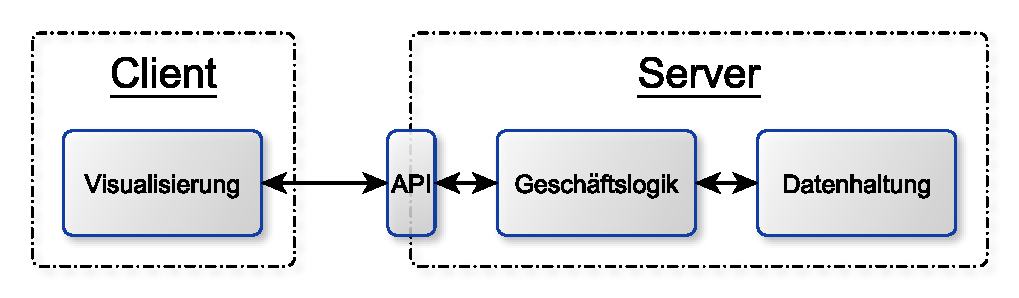
\includegraphics[width=0.75\textwidth]{img/konzeption/gesamtkonzept/Architektur.pdf}
  \captionsetup{format=plain,justification=centering}
  \caption[Architekturmodell]{Architekturmodell \\ \quelle Eigene Darstellung}
  \label{img:einkaufBPMN}
\end{figure}

Grundlegend ist deshalb die Architektur dem \ac{MVC}-Konzept nachempfunden, da der Server das Model durch die vorhandene Datenbank und die darin vorhandenen Relationen darstellt sowie die View des Konzepts durch den Client repräsentiert wird.
Der Controller wird dabei zu einem Teil durch die Geschäftslogik im Server und der damit verbundenen \ac{API} repräsentiert.
Zum anderen ist dieser jedoch ebenso im Client durch eine Sammlung und Aufarbeitung der Daten sowie einer geringfügigen Überprüfungen der Nutzereingaben vorhanden.\autocite{rf-leff2001web}

% !TEX root =  ../../master.tex
\section{Server}

\textcolor{red}{\textbf{Hier könnte der Aufbau von Docker hin...}}

% !TEX root =  ../server.tex
\subsection{Geschäftslogik}
% !TEX root =  ../server.tex
\subsection{Datenhaltung}
% !TEX root =  ../server.tex
\subsection{Schnittstellen}


% !TEX root =  ../../master.tex
\section{Client}

\subsection{Unterteilung der Gliederungsansichten}

	- Beschreibung der Mockups
		- Was haben wir uns bei den einzelnen Seiten gedacht
		- Wie sollten die Seiten grundsätzlich aussehen. (Brainstorming)
		- evtl. bissel auf Designthinking eingehen
		- Welches tool haben wir dazu genutzt
	- Recherche zu vorhandenen Umfragetools --> (https://www.polly.ai/slack-poll, https://strawpoll.de/, https://www.limesurvey.org/de/, https://www.surveymonkey.de/, https://pingo.coactum.de/)
		--> Ideensammlung und Marktrecherche
	- Grundlegende Idee der Einfachheit (evtl Gesamtkonzept)
	- Man könnte auf den User Journey eingehen
	- Anlehnung an DHBW farben sind vorgesehen
	- Orientierung an modernen Websites mit header und footer
	- Hinblick auf mobile usage
	
\subsection{Bestimmung von Darstellungsformen}
% !TEX root =  ../../master.tex
\section{Sicherheit}

% TODO: sollte zum Konzept verschoben werden, section gelöscht

% !TEX root =  ../sicherheit.tex
\subsection{Kommunikation}

\subsubsection{Transferprotokoll}\label{chapter:https}

Um die Sicherheit während der Kommunikation zu erhöhen dürfen Anfragen an den Webserver der Anwendung ausschließlich über \ac{HTTPS} zugelassen werden, sodass  die Kommunikation zwischen Server und Client verschlüsselt wird.
Dies stellt die Integrität der Daten sicher und erhöht damit ebenfalls ihre Vertraulichkeit.
Diese zwei Schutzziele dienen dazu einen potentiellen Angriff, wie etwa einen \ac*{MITM}-Angriff oder einen Lauschangriff, zu verhindern, indem das Ausspähen des Inhalts der Kommunikationspakete durch die vorhandene Verschlüsselung verhindert wird oder etwaige Veränderung der Pakete durch eine fehlerhafte Ent- und erneute Verschlüsselung bemerkt wird.

Zur Verschlüsselung verwendet \ac{HTTPS} die \ac{TLS} und unterscheidet sich grundlegend, neben der \ac{URL}, welche bei der Verwendung von \ac{HTTPS} mit \enquote{https://} beginnt, und der standardmäßigen Nutzung des Port 443, nicht weiter von \ac{HTTP}.

\ac{TLS} setzt dabei auf eine asymmetrische Verschlüsselung, wobei im ersten Schritt ein Schlüsselaustausch zwischen Client und Server vorgesehen ist.
Dies geschieht nach der Version \ac{TLS} 1.3 über drei verschiedene Wege, die aufgrund ihrer Zukunftssicherheit ausgewählt wurden.
Diese Zukunftssicherheit dient dazu, auch langfristige Angriffe zu verhindern, da so nicht alle potentiell von einem Angreifer abgefangenen \ac{TLS}-Sessions entschlüsselt werden können, sobald der private Schlüssel einer Session gefunden wurde.\autocite{rf-RFC8446}



\chapter{Implementierung}
\label{ch:implementierung}
% !TEX root =  ../../../master.tex
\subsection{Docker}
\label{sec:grundlagen:docker}
Bei der heutigen Softwareentwicklung spielt die Art und Weise, wie eine Software bereitgestellt wird, eine zentrale Rolle.
Gerade bei der Entwicklung einer verteilten Architektur wie die der Microservices (siehe Kapitel~\ref{sec:grundlagen:microservices}) ist dies besonders wichtig, da die einzelnen Schritte dieses Prozesses weitestgehend automatisch durchgeführt werden sollen.
Weiterhin benötigen Microservices in der Regel nur sehr wenige Hardware-Ressourcen und arbeiten autonom.
Aus diesen Gründen ist es sinnvoll, die vorhandenen Ressourcen eines Servers zu verteilen und gleichzeitig eine isolierte Umgebung für die einzelnen Microservices zu schaffen.

Hierbei hat sich in den letzten Jahren die Technologie \emph{Docker} besonders etabliert.
Docker ist eine von dem Unternehmen \emph{Docker, Inc.} entwickelte Software, welche eine Art der Container-Virtualisierung ermöglicht.
Die Software baut dabei auf einer Vielzahl von Open-Source-Projekten auf.

Die Container-Virtualisierung ist eine leichtgewichtige und ressourcenschonende Variante der Virtualisierung von Arbeitsumgebungen für Anwendungen.
Im Gegensatz zu virtuellen Maschinen bilden Container kein eigenständiges System ab, welches über virtuelle Hardware und ein vollständiges Betriebssystem verfügt.
Vielmehr wird eine isolierte Umgebung für eine spezifische Anwendung zur Verfügung gestellt, welche die Ressourcen des zugrundeliegenden Systems verwenden.

\begin{figure}[h]
	\centering
	\captionsetup{justification=centering, format=plain}
	\subfigure[Container-Virtualisierung]{\includegraphics[width=0.45\textwidth]{img/grundlagen/technisch/docker_container}}\hspace{1cm}
	\subfigure[Virtuelle Maschine]{\includegraphics[width=0.45\textwidth]{img/grundlagen/technisch/docker_hypervisor}}
	\caption[Vergleich Container-Virtualisierung vs. virtuelle Maschine]{\label{fig:docker_container}Vergleich Container-Virtualisierung vs. virtuelle Maschine, \\\quelle \cite{MS-DockerInc..05.03.2019}}
\end{figure}

Abbildung~\ref{fig:docker_container} visualisiert die Architektur einer Container-Virtualisierung und zeigt einen Vergleich zur Hardware-Virtualisierung.\autocite[Vgl.][]{MS-ChrissiKraus.27.07.2018}\autocite[Vgl.][]{MS-MicrosoftCorporation.31.08.2018}
Wie zu sehen ist, setzt Docker auf dem zugrunde liegenden Betriebssystem auf, wohingegen eine virtuelle Maschine als Gast-System agiert.
Dabei verwaltet und verteilt bei virtuellen Maschinen ein Hypervisor die Ressourcen, welche die Gast-Systeme zur Verfügung gestellt bekommen.
Ein Hypervisor ist also ein Manager für virtuelle Maschinen.\autocite[Vgl.][]{MS-ReneBust.06.04.2010}
Docker-Container bekommen hingegen ihre Ressourcen vom zugrunde liegenden Betriebssystem bereitgestellt.

Vorteile von Docker sind zum einen das hohe Maß an Integration und zum anderen eine gute Skalierbarkeit von Anwendungen.
Dabei können die Docker-Container sehr einfach erzeugt, gestartet und gestoppt werden.
Als Kern- und Steuerprogramm von Docker fungiert die sogenannte \emph{Docker Engine}.
Sie ist neben dem Starten und Stoppen in der Lage, vorhandene Container zu replizieren bzw. die Anzahl an Containern für einen speziellen Dienst bei Bedarf beliebig zu erhöhen oder zu verringern.
Hierzu kommt das Nebenprodukt \emph{Docker Compose} zum Einsatz.
Dieses Werkzeug dient dem Erzeugen von Multi-Container-Anwendungen.
Der Integrationsaspekt entsteht dadurch, dass Docker mit anderer Software interagieren bzw. sich von dieser steuern lassen kann.\autocite[Vgl.][]{MS-Docker-Compose}

% !TEX root =  ../../master.tex
\section{Server}

\textcolor{red}{\textbf{Hier könnte der Aufbau von Docker hin...}}

% !TEX root =  ../server.tex
\subsection{Geschäftslogik}
% !TEX root =  ../server.tex
\subsection{Datenhaltung}
% !TEX root =  ../server.tex
\subsection{Schnittstellen}


% !TEX root =  ../../master.tex
\section{Client}

\subsection{Unterteilung der Gliederungsansichten}

	- Beschreibung der Mockups
		- Was haben wir uns bei den einzelnen Seiten gedacht
		- Wie sollten die Seiten grundsätzlich aussehen. (Brainstorming)
		- evtl. bissel auf Designthinking eingehen
		- Welches tool haben wir dazu genutzt
	- Recherche zu vorhandenen Umfragetools --> (https://www.polly.ai/slack-poll, https://strawpoll.de/, https://www.limesurvey.org/de/, https://www.surveymonkey.de/, https://pingo.coactum.de/)
		--> Ideensammlung und Marktrecherche
	- Grundlegende Idee der Einfachheit (evtl Gesamtkonzept)
	- Man könnte auf den User Journey eingehen
	- Anlehnung an DHBW farben sind vorgesehen
	- Orientierung an modernen Websites mit header und footer
	- Hinblick auf mobile usage
	
\subsection{Bestimmung von Darstellungsformen}

\chapter{Nutzerhandbuch}
\label{ch:nutzerhandbuch}
% !TEX root = master.tex
\section{User Journey}

\chapter{Ausblick}
\label{ch:ausblick}
% !TEX root =  ../../master.tex
\section{Fazit zur Gruppen- und Seminararbeit}
\label{sec:Fazit}

Bei der Arbeit handelt es sich um die Dokumentation der Verwendung und Neuentwicklung einer Webanwendung.
Von den verwendten Grundlagen, sowohl aus technischer als auch theoretischer Sicht, bis hin zu einem Nutzerhandbuch, wurden alle Schritte zur Erstellung der Anwendung beschrieben.

Im Rahmen dieser Seminararbeit wurde eine Webanwendung zur Umfrageerstellung, -verwaltung und -ausführung erstellt.
Dazu wurden zunächst alle verwendeten Grundlagen, sowohl aus technischer als auch theoretischer Sicht, erläutert.
Anschließend wurde die Konzeption der Webanwendung beschrieben.
Dabei wurde die Client-Server-Architektur näher erläutert.
Dazu wurde im Bereich des Servers auf die Gestaltung der zugrundeliegenden Datenbank und der \acp{API} in einer \ac{REST}-Struktur eingegangen.
Zudem wurden erste Mock-Ups der Benutzeroberfläche entworfen und vorgestellt, die einen Anhaltspunkt für die Implementierung geliefert haben.
Weiterhin wurden wesentliche Punkte bezüglich sicherheitskritscher Aspekte, nämlich der Authentifizierung sowie der Autorisierung und dem zu verwendeden Transferprotokoll, verdeutlicht.
Dem folgt die Implementierung, welche die zuvor geschriebene Konzeption mit Hilfe der Front-End-Bibliothek \emph{React} zur Visualisierung und der JavaScript-Laufzeitumgebung \emph{Node.js} und dem Framework \emph{Express} verwirklicht wurden.
Zu guter Letzt wird die Benutzung der Software durch ein \emph{Nutzerhandbuch} sehr detailliert erläutert, sodass jegliche Funktionalität, die vom Nutzer verwendet werden kann, beschrieben wird.

Dadurch konnten alle zu Beginn der Arbeit beschriebenen und gestellten Anforderungen an die Applikation erfüllt werden.
Mithilfe der erstellten Software, welche durch Docker einfach bereitzustellen ist, können Umfragen erstellt, verwaltet und ausgewertet werden.
Dozenten können dies entsprechend nutzen, um die Interaktivität und den Abwechslungsreichtum von Vorlesungen zu steigern.
Gleichzeitig können Studierende über die angebotene Plattform an Umfragen teilnehmen, was bei korrekter Nutzung des Systems als Datengrundlage für Learning Analytics verwendet werden kann.
Darüberhinaus können auch Studenten solche Umfragen für ihre Bachelorarbeit mit Hilfe der Applikation erstellen.

Durch das Zusammenspiel eines etablierten Teams, welches sich in den vergangenen drei Jahren entwickelte, wussten die beteiligten Autoren, dass sie sich aufeinander verlassen können.
Ferner kannte jeder Student die Stärken und Schwächen der jeweils anderen.
Nur so konnte die bis jetzt entwickelte Anwendung auf ein solches Niveau gehoben werden.

Zu Beginn war es für manche Teammitglieder schwer, sich mit diesem Projekt zu identifizieren, da bereits andere Plattformen wie \enquote{Moodle} potenzielle Features möglich machen.
Jedoch fand das Team schnell einen gemeinsamen, ganzheitlichen Ansatz zum Entwickeln einer solchen Applikation.
Gemeinsam wurden Datenbankentwürfe erstellt und auf deren Richtigkeit überprüft.
Es wurden Konzepte erstellt, wie es möglich ist, eine geeignet Umfrage-Applikation zu entwerfen, die es möglich macht, individuelle Umfragen zu erstellen und diese anschließend graphisch darzustellen.
Gemeinsam mit den Stakeholdern wurden die Anforderungen besprochen.

Auch bedingt durch die Corona-Krise haben sich die Autoren nicht beeinträchtigen lassen. 
Vielmehr wurde hierdurch der Teamspirit gestärkt. 
Dies zeigte sich \ua dadurch, dass das Team auch auf Dinge verzichtete und eine Vielzahl an Mehrstunden in Kauf nahm, um das Projekt zu dem zu machen was es nun ist. 

% !TEX root =  ../../master.tex
\section{Ausblick}
\label{sec:Ausblick}

Die Anwendung hat zum aktuellen Stand noch ein großes Potenzial für Erweiterungen und Optimierungen.
Sie zeigt derzeit einen soliden Stand mit dem Hauptaugenmerk des Erstellens von Umfragen von verschiedenen Benutzern.

Es erscheint sinnvoll, der Applikation eine Art Forum, ähnlich einem Diskussionsforum, anzufügen.
Hintergrund ist, dass \zb Dozenten wie \dutzi ein Forumseintrag erstellen können, um hier Diskussionen zu führen.
So könnten die Teilnehmer aus dem Kurs wie \weigert über die Fragestellung diskutieren.
Andererseits könnten sich Studierende dort auch über verschiedene Themenbereiche zur Prüfungsvorbereitung austauschen und hier Dokumente teilen. \newline
Um dies zu realisieren, müssten Datenbankanpassungen vorgenommen werden, damit das Forum dargestellt werden kann und auch Studenten einen Benutzer mit Systemzugang erhalten.

% - Back-End hat bereits weitere Funktionen implementiert, die nun nach und nach im Front-End nachgezogen werden können
Das Back-End wurde bereits um eine Vielzahl an Funktionen ergänzt, welche lediglich im Front-End nachgezogen werden müssen.
Dazu zählen, dass:
% 
\begin{itemize}
    \item Umfragevorlagen \zb nach Vorlesungen gruppiert,
    \item Kommentare zu Umfragen hinzugefügt, 
    \item Start- und Endzeitpunkt von Umfragen festgelegt
    \item und Umfragevorlagen und Fragen öffentlich als Template für andere zur Verfügung gestellt
\end{itemize}
% 
werden können.

Die Anwendung wurde ganzheitlich in englischer Sprache umgesetzt.
Sie könnte mittels Internationalisierung effizient um die Unterstützung weiterer Sprachen erweitert werden.
Dazu muss lediglich für jede Sprache eine Datei angelegt werden, die die Übersetzungen der einzelnen verwendeten Textbausteine auflistet.
Neben einem manuellen Wechsel der Sprache kann hier standardmäßig die vom Benutzer präferierte Sprache angezeigt werden, wenn dieser seinen Webbrowser bzw. sein System entsprechend eingestellt hat.

Zur Optimierung der Auswertung wäre es von Nutzen, Umfrageergebnisse, die auf derselben Vorlage beruhen, miteinander zu vergleichen.
Dies umfasst auf der einen Seite die Darstellung des zeitlichen Verlaufs von Umfrageergebnissen, die wiederholt in einem Kurs durchgeführt werden (Panel).
Auf der anderen Seite können ebenfalls mehrere Kurse untereinander verglichen werden.

Ein zusätzliches Feature der Anwendung wäre das Speichern und Exportieren der Resultate zur weiteren Verarbeitung im \acs{CSV}- oder \acs{PDF}-Format.

Des Weiteren könnte eine Ergänzung weitere Informationen rund um die Umfrage und deren Resultate beinhalten.
So könnte etwa ein Stichprobenrechner hilfreich sein, um den benötigten Stichprobenumfang einer Umfrage zu errechnen, sodass die Umfrage als repräsentativ im gewünschten Fall zu bewerten ist.
Dabei werden Kennzahlen wie die Größe der Grundgesamtheit, das Konfidenzniveau und die Fehlermarge als Errechnungsgrundlage benötigt.
In diesem Zusammenhang können auch direkt die Auswertungsoptionen im Front-End um weitere Diagrammtypen erweitert werden.


% bibliography
\clearpage
\ihead{}
\printbibliography[title=Literaturverzeichnis]
\cleardoublepage

% appendix
\appendix
\ihead{\appendixname~\thechapter}

% !TEX root =  ./master.tex
\chapter{Abbildungen}

\begin{sidewaysfigure}[ht]
	\centering
	\def\svgscale{0.85}
	\graphicspath{{img/backend/database/}}
	\scriptsize{\input{img/backend/database/er-myla-2020-06-04.pdf_tex}}
	\caption{\acs{ER-Modell}}
	\label{fig:er-model}
\end{sidewaysfigure}

\begin{figure}[h]
	\centering
	\includegraphics[width=0.7\textwidth]{img/konzeption/client/umfrage_erstellen_multiple_choice}
	\captionsetup{justification=centering, format=plain}
	\caption[Mock-Up der Umfrageerstellung von Multiple-Choice-Fragen]{Mock-Up der Umfrageerstellung von Multiple-Choice-Fragen \\\figma}
	\label{fig:MockUmfrageMultipleChoice}
\end{figure}

\begin{figure}[h]
	\centering
	\includegraphics[width=0.7\textwidth]{img/konzeption/client/umfrage_erstellen_rating}
	\captionsetup{justification=centering, format=plain}
	\caption[Mock-Up der Umfrageerstellung von Rating-Fragen]{Mock-Up der Umfrageerstellung von Rating-Fragen \\\figma}
	\label{fig:MockUmfrageRating}
\end{figure}


% ewerkl.tex
%% !TEX root =  master.tex

\clearpage
\chapter*{Ehrenwörtliche Erklärung}

Wir versichern hiermit, dass wir die vorliegende Arbeit
 mit dem Thema: \textit{\DerTitelDerArbeit} selbstständig verfasst und keine anderen als die angegebenen Quellen und
Hilfsmittel benutzt haben. Wir versichern zudem,
dass die eingereichte elektronische Fassung mit der gedruckten Fassung übereinstimmt.

\vspace{2cm}
Mannheim, den 14.02.2019

\vspace{10mm}
\authorSG
\hfill \authorRF
\hfill \authorGP

\vspace{5mm}
\hfill \authorEJ
\hfill \authorNL
\hfill
\clearpage
\includepdf[pages={1}]{ewerkl-signed.pdf}


\end{document}
